\section{Resultados}

\subsection{Requisito 1}

Implementou-se 3 classes no total e consistem em:


\begin{itemize}
\item Ponto: Uma alternativa em vez de passar as coordenadas x e y frequentemente, com risco de troca entre os termos.
\item Pixel: Para armazenar as componentes RBG de um pixel. Fez-se essa classe para evitar passar as 3 componentes frequentemente
\item Imagem: Para armazenar a imagem e abrigar metodos de pintar certos pixeis, a de pintar todos de mesma cores, e descobrir se imagem é na escala cinza.
\end{itemize}

 A partir dessas classes, a implementação do algoritmo que atendesse ao requisito 1 consistiu em: A cada momento que fosse clicado em um ponto difente, a função responsável pelo mouse retornava as coordenadas $(x, \ y)$ do ponto clicado. Em um loop, sempre que o ponto era diferente do ponto clicado anteriormente, passa-se o ponto $(x, \ y)$ para o objeto da imagem e captura as informações e imprime na tela.

Os resultados são mostrados pelas Figuras (\ref{fig:re1color}) e (\ref{fig:re1gray})

\begin{figure}[!ht]
\centering
\label{fig:re1color}
\caption{Requisito 1 - Imagem colorida}
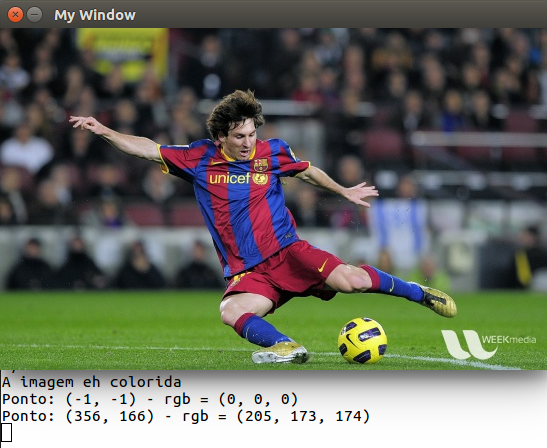
\includegraphics[width=0.5\textwidth]{img/T1_colored.png}
\end{figure}

\begin{figure}[!ht]
\centering
\label{fig:re1gray}
\caption{Requisito 1 - Imagem escala cinza}
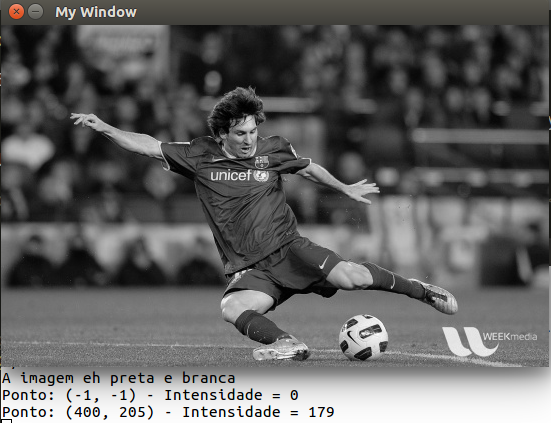
\includegraphics[width=0.5\textwidth]{img/T1_grayscale.png}
\end{figure}

\subsection{Requisito 2}

Para o requisito 2, bastava apenas pegar a informação coletada no requisito 1 e colorir pixeis próximos.
Para isso, bastou implementar a função \textit{PintaDistancia} em que colore todos os pixeis próximos de acordo com a distância. Mudando o parâmetro \textit{distancia}, na linha 54 dos algoritmos 2.cpp, 3.cpp e 4.cpp, obtém-se diferentes resultados.

Um fator a ser comentado é que sempre que há mudança do ponto clicado, a imagem é recarregada e colorida conforme o pixel clicado. Dessa maneira, sempre se espera um evento de clique para recarregar a imagem e pintar. O resultado é mostrado pela Figura (\ref{fig:re2colored})

\begin{figure}[!ht]
\centering
\label{fig:re2colored}
\caption{Requisito 1 - Imagem escala cinza}
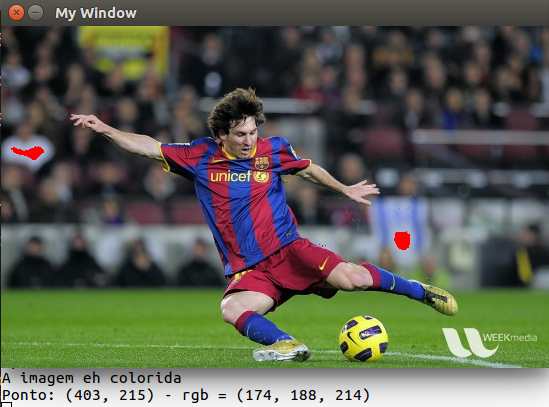
\includegraphics[width=0.5\textwidth]{img/T2_colored.png}
\end{figure}

\subsection{Requisito 3}

Conforme comentado na metodologia, de que o objetivo de implementação desse requisito era fazer a mudança apenas do frame e utilização de uma referência de pixel, obteve-se o resultado esperado.

Infelizmente não foi possivel fazer a troca do video para preto e branco pois a função testada e mostrada pela literatura\cite{cvtColor} não funcionada embora diversas tentativas de adaptação.

\subsection{Requisito 4}

Fazendo os processos descritos na metodolia, obteve-se o código implementando no arquivo 4.cpp em que se utiliza a câmera para captura de imagens.


